\subsection{Radiative Cooling and Heating}
\label{sec.num.cooling}

\enzo\ has multiple methods for computing the energy change from radiative
cooling and heating.  All of them assume the gas can be modeled either as
completely optically thin or with a simple, local approximation to optical
thickness.  Below we describe the methods for computing the cooling rates from
metal-free and metal-enriched gas.  Sample cooling curves for each of \enzo's
primary cooling methods are shown in Figure \ref{fig.cooling_rate}.

\subsubsection{Primordial Cooling}

As discussed in Section~\ref{sec.num.chemistry}, the set of reactions that
characterize a metal-free gas is simple enough to be computed in
non-equilibrium during even very large simulations.  Similarly, the radiative
cooling of metal-free gas is solved by directly computing the cooling
and heating rates from the following individual processes for atomic H
and He: collisional excitation and ionization, recombination,
free-free emission, Compton scattering off of the cosmic microwave
background (CMB), and photo-heating from a UV metagalactic background.
If the \HH chemistry network is enabled, the following \HH
cooling processes are also considered: ro-vibrational transitions
\citep{2008MNRAS.388.1627G,1998A&A...335..403G}, heating and cooling from molecular
formation and destruction \citep{2009Sci...325..601T}, and
collision-induced emission \citep{2004MNRAS.348.1019R}.  If Deuterium
chemistry is enabled, then rotational transitions of HD
\citep{1998A&A...335..403G, 1983ApJ...270..578L} are treated as well.  The
radiative cooling calculation is coupled to the update of the chemistry network
such that they both occur within the same subcycling loop.  This is necessary
in regimes where rapid cooling or change in the ionization state occur, as this
will influence the chemical kinetic rate coefficients through both changes in
energy and the equation of state of the gas.  In addition to the subcycle
timestepping contraints mentioned in Section~\ref{sec.num.chemistry}, the
subcycle timestep is also not permitted to exceed 10\% of the cooling time,
$t_{cool} = e/\dot{e}$.  A metagalactic background affects the gas through both
photo-heating and photo-ionization.  These are treated by including
redshift-dependent photo-ionization and photo-heating rate terms in the
chemistry and cooling equations for \ion{H}{1}, \ion{He}{1}, and \ion{He}{2}.
The black curves in Figure \ref{fig.cooling_rate} show cooling rates for a
metal-free gas with number density $n_{\rm H} = 10^{-4}$ cm$^{-3}$ both with
and without a radiation background.  More detail on the specific UV backgrounds
present in \enzo\ is presented below in Section~\ref{sec.num.rad-homogeneous}.

\subsubsection{Metal Cooling}

A proper treatment of the cooling from metals is significantly more
challenging due to the large number of chemical reactions and energy
transitions that must be taken into account for each element.  Because
of this, most metal cooling methods employ significant assumptions in
order to seek out a balance between accuracy and speed.  There are two
primary metal cooling methods available in \enzo.  The simpler of the
two uses the analytic cooling function of \citet{SW87}, which assumes
a fully ionized gas with a constant metallicity of 0.5 Z$_{\odot}$.
The cooling rate produced by this cooling function is shown by the red 
curve in Figure \ref{fig.cooling_rate}.

A more sophisticated method makes use of multidimensional cooling and
heating rate tables computed with the photo-ionization code
\texttt{Cloudy} \citep{1998PASP..110..761F}.  This method, detailed in
\citet{2008MNRAS.385.1443S} and \citet{2011ApJ...731....6S}, works by
using \texttt{Cloudy} to compute the cooling and heating rates from
the metal species only.  The primary assumption made is that of
ionization equilibrium.  The tables can vary along up to five dimensions,
of density, metallicity, electron fraction,
redshift (for an evolving metagalactic UV background), and
temperature.  Tables can be created for any abundance pattern for
elements up to atomic number 30 (Zn) and for any incident radiation
field.  Cooling from the standard \enzo\ non-equilibrium cooling module is
applied on top of the metal contributions.  The contribution of metals
to the cooling is computed within the same subcycling loop as the
coupled primordial chemistry and cooling solver.  The blue curves in
Figure \ref{fig.cooling_rate} show cooling rates calculated with this
method for a gas with number density $n_{\rm H} = 10^{-4}$ cm$^{-3}$ and
metallicity of 0.5 Z$_{\odot}$.

\begin{figure}
  \begin{center}
    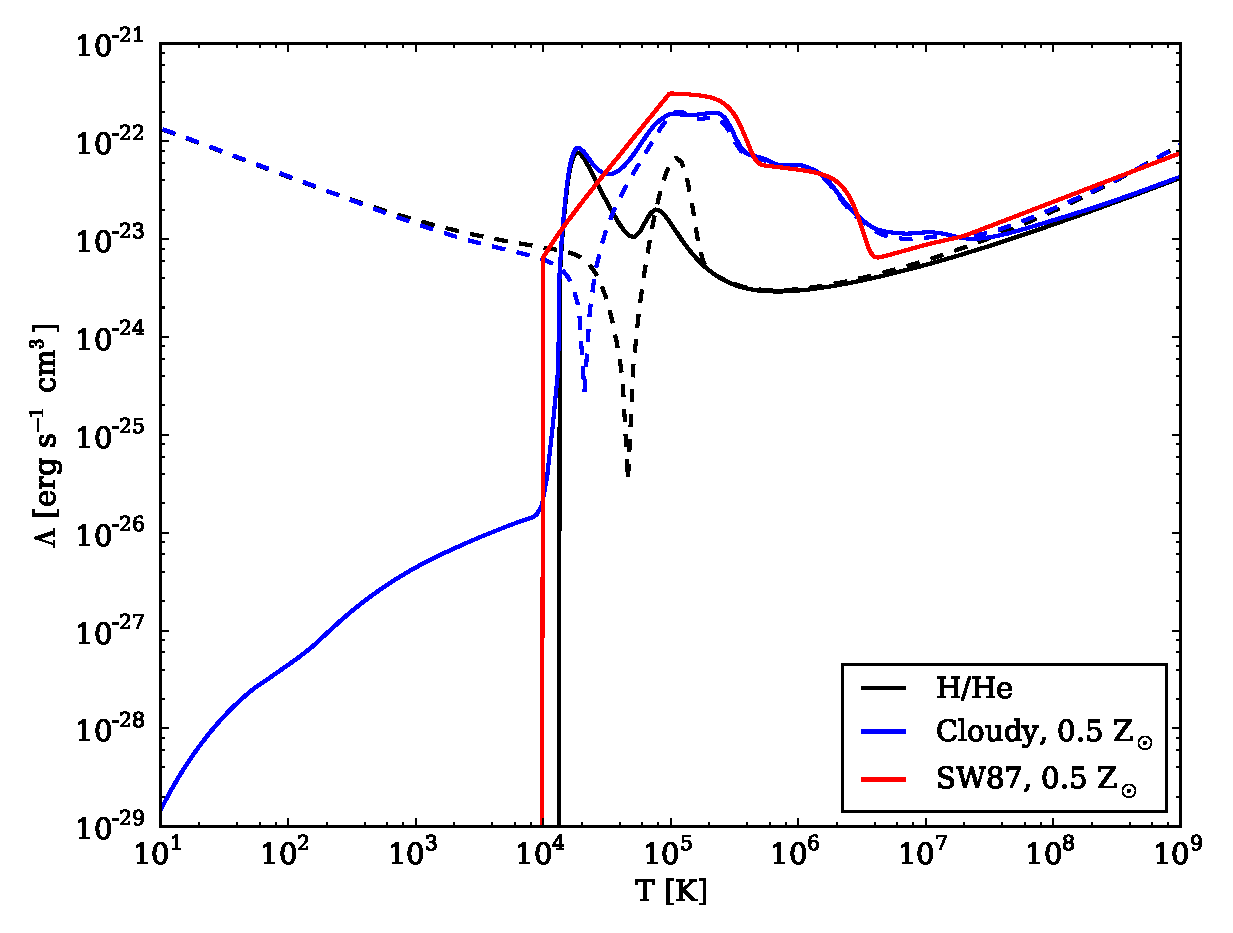
\includegraphics[width=1.0\textwidth]{figures/cooling_rate.eps}
  \end{center}
  \caption{Radiative cooling rates from the various cooling methods
    available in \enzo.  The black curves show cooling rates from a gas
    with primordial composition using the non-equilibrium chemistry
    network.  The blue curves are for a gas with metallicity of 0.5
    $Z_{\odot}$ computed with the Cloudy cooling method.  The solid
    black and blue lines assume collisional processes only while the
    dashed lines include photo-ionization and photo-heating from a UV
    metagalactic background at $z = 0$ with a gas number density of
    10$^{-4}$ cm$^{-3}$.  The rates shown by the
    dashed lines indicate a net heating below $T \sim 10^{4.5}$, where
    the rapid change in rate is evident (the curve is an absolute
    value so it can be shown on a log plot).  The red curve is the
    tabulated cooling function of \citet{SW87}, which assumes a fully
    ionized gas with metallicity of 0.5 $Z_{\odot}$.}
  \label{fig.cooling_rate}
\end{figure}
